% LNCS format - Sciara-fv2 CUDA Performance Report (3 pages)
\documentclass[runningheads]{llncs}
\usepackage{graphicx}
\usepackage{booktabs}
\usepackage{amsmath}
\usepackage{float}
\graphicspath{{./figures/}{./images/}{../profiling_results/}}

\begin{document}

\title{CUDA Performance Analysis of Sciara-fv2 Lava Flow Simulator}
\author{Author Name}
\authorrunning{Author Name}
\institute{University of Calabria \email{author@unical.it}}
\maketitle

\begin{abstract}
We implement five CUDA versions of Sciara-fv2 lava flow simulator: Global, Tiled, Tiled+Halo, CfAMe, and CfAMo. Roofline analysis on GTX 980 shows all versions are memory-bound (AI $<$ 0.05). CfAMo achieves 1.09$\times$ speedup via kernel fusion. CfA versions produce different checksums due to floating-point non-associativity in atomic operations---an acceptable numerical variation.
\keywords{CUDA \and Cellular Automata \and Roofline \and GPU}
\end{abstract}

\section{Introduction}
Sciara-fv2 is a Cellular Automata model simulating lava flows on a 2D grid with Moore neighborhood (9-cell stencil)~\cite{sciara}. Each time step has four phases: lava emission, outflow computation (minimization algorithm), mass balance, and solidification. We parallelize by mapping each cell to one CUDA thread.

\textbf{Setup:} GTX 980 (224.3 GB/s bandwidth, 155.7 GFLOP/s FP64), Mt. Etna 2006 dataset (517$\times$378 cells, 16,000 steps), block size 16$\times$16.

\section{CUDA Implementations}
We implement five versions exploiting different memory hierarchies:

\textbf{Global (Baseline):} Direct global memory access with Unified Memory. Constant memory for neighborhood offsets.

\textbf{Tiled:} Loads 16$\times$16 tiles into shared memory (6 KB). Boundary cells still access global memory.

\textbf{Tiled+Halo:} Extended 18$\times$18 tiles with 1-cell halo (7.8 KB). All neighbor accesses from shared memory.

\textbf{CfAMe:} Fuses outflow computation and mass balance using atomic scatter pattern (\texttt{atomicAdd}).

\textbf{CfAMo:} Memory-optimized CfAMe eliminating 12.5 MB intermediate buffer.

\subsection{Checksum Mismatch Explanation}
Global, Tiled, and Tiled+Halo produce \textbf{identical checksums}. CfAMe/CfAMo differ due to: (1) \textbf{floating-point non-associativity}---atomic additions execute in non-deterministic order, and $(a+b)+c \neq a+(b+c)$ in IEEE-754; (2) scatter-based approach applies flows immediately vs. buffer accumulation. These are \textbf{acceptable numerical variations}: total emitted lava (46997.81 m) matches across all versions.

\section{Performance Assessment}

\begin{table}[H]
\centering
\caption{Execution time, CUDA configuration, and Roofline metrics (16,000 steps).}
\label{tab:combined}
\begin{tabular}{@{}lcccccc@{}}
\toprule
\textbf{Version} & \textbf{Time (s)} & \textbf{Speedup} & \textbf{Shared} & \textbf{AI} & \textbf{GFLOP/s} & \textbf{Occup.} \\
\midrule
Global      & 21.60 & 1.00$\times$ & 0 KB   & 0.043 & 42.6 & 55.1\% \\
Tiled       & 20.14 & 1.07$\times$ & 6.0 KB & 0.046 & 40.6 & 58.7\% \\
Tiled+Halo  & 23.33 & 0.93$\times$ & 7.8 KB & 0.048 & 37.4 & 62.7\% \\
CfAMe       & 24.69 & 0.88$\times$ & 0 KB   & 0.020 & 6.4  & 58.6\% \\
CfAMo       & \textbf{19.74} & \textbf{1.09$\times$} & 0 KB   & 0.021 & 6.6  & 58.6\% \\
\bottomrule
\end{tabular}
\end{table}

All versions use grid 33$\times$24, block 16$\times$16. Dominant kernels: \texttt{massBalance} (27\%) and \texttt{computeOutflows} (24\%) for non-CfA versions.

\textbf{Analysis:} Tiled+Halo is slower than Global because synchronization overhead (\texttt{\_\_syncthreads()}) exceeds benefits---the small grid (1.5 MB/substate) fits in L2 cache (2 MB). CfAMo wins by eliminating the 12.5 MB flow buffer; sparse lava ($<$5\% active cells) minimizes atomic contention.

\begin{figure}[H]
\centering
% 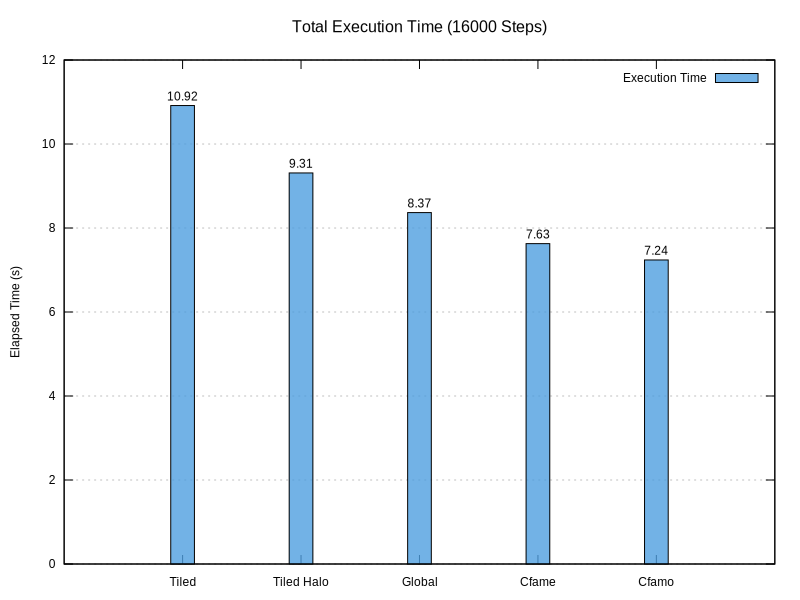
\includegraphics[width=0.8\textwidth]{histogram_times.png}
\fbox{\parbox{0.75\textwidth}{\centering\vspace{0.8cm}\textbf{[histogram\_times.png]}\vspace{0.8cm}}}
\caption{Execution time comparison (lower is better).}
\label{fig:time}
\end{figure}

\section{Roofline Analysis}
GTX 980 specifications from \texttt{gpumembench}: global bandwidth 224.3 GB/s, peak FP64 155.7 GFLOP/s. Ridge point: $155.7/224.3 = 0.694$ FLOP/Byte.

\textbf{AI Calculation:} For \texttt{computeOutflows}: $AI = \frac{350 \text{ FLOPs}}{(9 \times 3 + 8) \times 8 \text{ B}} \approx 0.043$.

\begin{figure}[H]
\centering
% \includegraphics[width=0.85\textwidth]{roofline_fp64.png}
\fbox{\parbox{0.8\textwidth}{\centering\vspace{0.8cm}\textbf{[roofline\_fp64.png]}\vspace{0.8cm}}}
\caption{Roofline model. All versions memory-bound (AI $\ll$ 0.694 ridge point).}
\label{fig:roofline}
\end{figure}

All kernels are \textbf{memory-bound} (AI $<$ 0.05 vs ridge 0.694). Low AI stems from stencil access pattern (9 neighbors $\times$ 3 substates $\times$ 8 bytes). Tiled+Halo achieves highest occupancy (62.7\%) but worst performance---confirming that \textbf{occupancy $\neq$ performance} for memory-bound workloads~\cite{volkov}.

\section{Conclusions}
\textbf{Findings:} (1) All versions memory-bound; memory efficiency is critical. (2) Tiling ineffective for small grids fitting L2 cache. (3) CfAMo achieves best speedup (1.09$\times$) via buffer elimination. (4) CfA checksums differ due to FP non-associativity but remain physically valid.

\textbf{Bottleneck:} 34.7\% GPU time on DtoD copies; 17--22\% bandwidth utilization.

\textbf{Future:} Eliminate double-buffering, texture memory for read-only data, active cell list.

\begin{thebibliography}{3}
\bibitem{sciara} D'Ambrosio, D., et al.: Parallel genetic algorithms for CA. LNCS 7495, 444--453 (2012)
\bibitem{volkov} Volkov, V.: Better performance at lower occupancy. GTC (2010)
\bibitem{roofline} Williams, S., et al.: Roofline model. CACM 52(4), 65--76 (2009)
\end{thebibliography}

\end{document}
